%\sorgt 	%ensures the apparition of "Appendix" before each appendix.
%\openany	%ensures that a chapter can begin on each side and not only on the right site.
%\bibtotoc	%ensures that the bibliography automatically appears in the table of contents.
%\documentclass[colordvi,11pt,a4paper,halfparskip,final,headings,appendixprefix,bibtotoc]{scrbook}
\documentclass[
	pdftex,
	chapterprefix,
	headsepline,
	footsepline,
	% colordvi,
	11pt,
	a4paper,
	parskip=half,
	final,
	appendixprefix,
bibliography=totoc]{scrbook}

% uncomment the following line (mutual exclusive to the one above) to enter the draft mode.
%\documentclass[colordvi,11pt,a4paper,halfparskip,draft,appendixprefix,bibtotoc]{scrbook}

\newcommand{\studentFirsName}{Michael}
\newcommand{\studentSecondName}{Krane}
\newcommand{\studentMatrikelnummer}{2233018}

% Define a new one if is possible to choose between PDF and DVI.
\usepackage{ifpdf}
\ifx\pdfoutput\undefined
\pdffalse %not PDFLaTeX
\else
\pdfoutput=1
\pdftrue
\fi
%\tracingstats=2
%\usepackage{layout}
% english/spanish/new german language support (hyphenation etc)
\usepackage[english]{babel}
\selectlanguage{english}

% for prettier tables
\usepackage{booktabs}

% support for latin1 characters. That means you can enter umlauts directly
% no need for "a "u "o "s anymore
\usepackage[ansinew]{inputenc}
%\usepackage[latin1]{inputenc}

% provides the \url{} command to pretty print urls
\usepackage{url}

% needed for a german bibliography-style (s. below)
\usepackage{bibgerm}

% allows text flowing around figures.
\usepackage{wrapfig}

% allows to \includegraphics
\usepackage{graphicx}

% defines some standard colornames like "black" etc.
\usepackage{color}

% allows to color tablecells
\usepackage{colortbl}

% provides an easier interface to if-then-else constructs in 
% custom macros
\usepackage{ifthen}

% allows tables to break over pages.
\usepackage{supertabular}

% allows to have different kinds paper orientations in the same pdf-documnent
\usepackage{pdflscape}

% allows to specify absolute texpos for textboxes. This is generally only important for the titlepage
\usepackage[absolute]{textpos}

% allows to enumerate different figures with a) b) in the same figure-environment.
\usepackage{subfigure}

\usepackage{float}

\usepackage{multirow}

\usepackage{listings}
\lstset {language = C,
		showspaces = false,		
		showstringspaces=false,		
		showtabs = false,
		basicstyle = \normalsize\ttfamily}

% finetune the gaps between figure and text in the subfigure environment (basically close the gap as much as possible)
\renewcommand{\subfigtopskip}{0pt}
\renewcommand{\subfigbottomskip}{0pt}

% some color definitions for the pdf statements below
\definecolor{mygrey}{rgb}{0.45,0.45,0.45}
\definecolor{mydarkgrey}{rgb}{0.2,0.2,0.2}
\definecolor{red}{rgb}{1.0,0.33,0.33}
\definecolor{orange}{rgb}{1.00,0.73,0.33}
\definecolor{yellow}{rgb}{0.95,0.92,0.}
\definecolor{lightgreen}{rgb}{0.3,0.95,0.46}
\definecolor{titleblue}{rgb}{0.03,0.10,0.46}

\ifpdf
% Metadata and configuration of the pdf output:
% Do not forget to enter the correct title, author, subject und keywords

% For the final printouts (remember - you need at least three - one for each examiner and one for the archive 
% [ This might have changed - so contact the "Pr�fungsamt" about the current regulations !! ] - it is better
% to have all text in the same color (namely black).
% 
\usepackage[pdftex,
            pdftitle={},
            colorlinks,
            linkcolor={black},
            citecolor={black},
            urlcolor={black},
            plainpages={false},
            bookmarksnumbered={true},
            pdfauthor={},
            pdfsubject={},
            pdfkeywords={},
            pdfstartview={FitBH}]{hyperref}
\pdfcompresslevel=9
\fi

% some configuration for the amount of text on a single page
\usepackage{typearea}
\areaset[1.5cm]{418pt}{658pt}
\setlength{\headheight}{37pt}

% Enter author and title for the titlepage.
\author{Michael Krane}
\title{Evaluation of a lightweight debugging platform for mobile sensor networks}

% To avoid nasty mistakes like having comments directly in the textflow
% the following \todo macro was defined. With that you can enter
% \todo{What I still have to do here} 
% inside of your text and a marker will appear at the page's margin with the 
% text "What I still have to do here".
% The first line activates this feature. If you comment it out and uncomment
% the second line below there will be no error messages and no todos will be shown
% anymore. So - even if you have forgotten to delete one of them - they will not appear
% in the final printout. 
%\newcommand{\todo}[1]{\marginpar{\textcolor{red}{ToDo:} #1}}
\newcommand{\todo}[1]{}

% We recommend to split your document into several files. Usually one for every chapter is a 
% good idea. If you follow this guideline (how to assemble these files in a single document
% see two paragraphs below) you will be able to single out chapters via the \includeonly{}
% command. Using this mechanism page numbering and references of the full run before will be
% preserved. This also nice, if your latex run tends to get slow and you need to fine tune 
% some formatting in one chapter - just include that one. The rest (or at least the ones before
% the one currently under construction) will remain untouched. This means a boost in compilation time.
%\includeonly{chapter2}

\begin{document}
\newfloat{code}{h}{bmccode}
\floatname{code}{Pseudo code}
% the next two lines influence the detailedness of the table of contents
% and to what structure depth numbers are written before sections/subsections/paragraphs
% You should not touch this
\setcounter{tocdepth}{2}
\setcounter{secnumdepth}{3}
\frontmatter
% here the titlepage is included. Look into the file "titlePage.tex" to 
% adapt it to your needs (name, title etc.)
% Titelseite braucht folgenden  Eintrag
% \usepackage[absolute]{textpos}
% textpos ist nicht Bestandteil von tetex
% kann aber von dante heruntergeladen werden
\begin{titlepage}
\vspace*{-1cm}
\newlength{\links}
\setlength{\links}{0.9cm}
\setlength{\TPHorizModule}{1cm}
\setlength{\TPVertModule}{1cm}
\textblockorigin{0pt}{0pt}

\sf
\LARGE

\begin{textblock}{16.5}(2.8,2.6)
 \hspace*{-0.25cm} \textbf{UNIVERSIT�T DUISBURG-ESSEN} \\
 \hspace*{-1.15cm} \rule{5mm}{5mm} \hspace*{0.05cm} FAKULT�T F�R WIRTSCHAFTSWISSENSCHAFTEN\\
 \large{}INSTITUT F�R INFORMATIK UND WIRTSCHAFTSINFORMATIK \\
 \large{}LEHRSTUHL F�R PERVASIVE COMPUTING\\
\end{textblock}


%Hier Titel, Name, und Matrikelnummer eintragen, \\ make a newline
\begin{textblock}{14.5}(3.2,8.5)
  \large
{ \bf Bachelorarbeit} \\[1cm]
{\LARGE \Large\bf Evaluation of a lightweight debugging platform for mobile	sensor networks} \\[1.3cm]
\studentFirsName { } \studentSecondName\\
Matrikelnummer: \studentMatrikelnummer
\end{textblock}



\begin{textblock}{10}(10.5,17.5)
%
\includegraphics[scale=1.0]{unilogo.pdf}\\

\includegraphics[scale=0.23	]{content/images/NES_Logo.pdf}\\
\normalsize
\raggedleft
Networked Embedded Systems Group \\
Institut f�r Informatik und Wirtschaftsinformatik \\
Fakult�t f�r Wirtschaftswissenschaften \\
Universit�t Duisburg-Essen \\[2ex]

\today\\[15ex]
\raggedright
% Pr�fers
{\bf Erstpr�fer:} Prof. Dr. Pedro Jos� Marr�n \\
{\bf Zweitpr�fer:} Prof. Dr. Gregor Schiele \\
{\bf Zeitraum:} 1.Juli 2015 - 29.September 2015\\
\end{textblock}


\end{titlepage}

\tableofcontents

\listoffigures
\mainmatter

% To assemble the whole document
% Please be aware that each file will begin on a new page
% therefore chapters should be put into such a file.
% There cannot be an include statement inside of an "included" file.
% So if you want to further divide your document - use \input inside of 
% the included files. \input will not begin on a new page.
%\setcounter{page}{2}

\cleardoublepage
\section*{Abstract}
In this thesis, we evaluate a component of SHAMPU(Single chip Host for Autonomous Mote Programming over USB), developed at the University of Duisburg-Essen. 
SHAMPU is a framework which allows the monitoring, debugging, and reprogramming of wireless sensor networks (WSN). 
Our focus for this evaluation is on the wireless communication between SHAMPU nodes, for which the ANT protocol is used. 
We designed and ran several different experiments in order to determine the capabilities of the ANT-chip in use.
\cleardoublepage

\chapter{Introduction}
\label{sec:intro}
In the present years the number of Cyber Physical Systems (CPSs) has drastically increased. This increase is mostly due to the emergence of the Internet of Things (IoT), as well as to the existence of several user friendly kits, auch as the RaspberryPi or the Arduino. With this recent trend new challenges are created in the monitoring and debugging of the above mentioned devices. This is especially difficult for applications, where the sensors are deployed in a hard to reach area. Moreover, sensors can often fulfill multi-purpose roles and might have to be reconfigured for different tasks.

In order to address both of these problems, SHAMPU(Single chip Host for Autonomous Mote Programming over USB)\cite{smeets2014demonstration} was developed at the University of Duisburg-Essen. SHAMPU is a design framework for monitoring and reprogramming WSNs. The main goal of SHAMPU is to be as small, lightweight and energy efficient as possible. Furthermore, a SHAMPU node is OS independent and can easily be attached to an existing node over USB. The SHAMPU nodes have multiple ways to transmit data between them, one of which is a wireless interface. In the current configuration, an ANT\cite{DynastreamInnovationsInc.2013} radio chip is used to transfer data between the SHAMPU nodes. Additionally, the nodes are connected to a base station which not only acts as a central data sink, but is also capable of pushing commands and data to the SHAMPU nodes. These wireless capabilities make it possible to remotely monitor, debug, and even reconfigure already deployed sensor nodes. 

In this thesis we evaluate the wireless capabilities of the SHAMPU framework. For that purpose we investigate use-cases for the different tasks the SHAMPU framework can perform: Program a device, collect data during operation, and interact with the system itself. For each of the use-cases we designed different experiments to assess how well ANT performs.
\newpage


\section{Related work}
\label{sec:related_work}
There are several different WSN test beds available. Each of these test beds is capable of monitoring and debugging an attached sensor node. The main difference between them is the size and specific role they were designed for. 

Some test beds like FlockLab \cite{Lim2013} allow to attach a wide array of different sensors and use a JTAG interface to be able to precisely capture debugging and timing information.

However, these types of test beds rely on a wired connection to interface with the test bed. Additionally, the platform itself has a large form factor. This makes it exceedingly difficult to test and debug already deployed WSNs since it might not be possible to easily get to the sensor in the planted location.

Other available solutions address this infrastructure dependency by attaching the test bed directly to the node and use a wireless connection to communicate with it. An example is Sensei-UU \cite{Rensfelt2009}, which uses a wireless 802.11 network. This set up allows the WSN to be tested and debugged while it is deployed. One drawback, however, is the power draw of 802.11 devices, which is huge compared to other technologies. To run the node itself on an external power source would not be a problem, but the use of a battery to power the node will hardly be feasible.

To address the power issue, it is possible to use a different technology which offers a lower power mode. Two examples are BTNodes \cite{Moser} or Smart-Its \cite{Kasten2000}, which use a Bluetooth connection. 
The structure of the network itself is similar to Sensei-UU: each node in the network has its own test bed attached and the test beds communicate with a central base station.

The main problem with Bluetooth is the limited size of the network, which makes it difficult to set up and use more complex network topologies. Also, Bluetooth communication is always 1:1 and does not allow broadcasts. The newest version of Bluetooth addresses the network size with the introduction of ScatterNets, but the setup and maintenance of the network remains challenging.

None of the above mentioned test beds exactly fit the design goals of SHAMPU. The test bed has to be directly attached to a fixed infrastructure, either because it has no wireless capabilities or because the power consumption is too high. BTNodes could be a possible alternative for SHAMPU. However Bluetooth connections are not well suited for the use in WSNs since they mostly use unicast.
	%Introduction
\chapter{Technical Background}
\section{SHAMPU}
SHAMPU\cite{smeets2014demonstration} is a design framework which allows remote debugging and reprogramming of sensor nodes. Its main advantages over other testbeds (see section~\ref{sec:related_work}) are portability, low cost, small size and low energy consumption. SHAMPU is used as an extension to an already existing sensor node. The only requirement is that the node provides an USB-Interface which is connected to SHAMPU. This single connection to the attached node makes SHAMPU OS independent.
\begin{figure}[H]
	\centering
	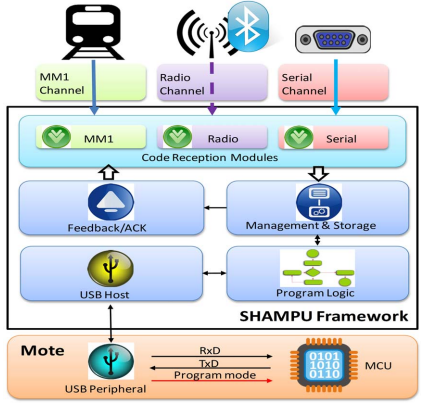
\includegraphics[scale=.5]{content/images/SHAMPUframework.png}
	\caption{Overview of the SHAMPU Framework \cite{smeets2014demonstration}}\label{fig:shampuframework}
\end{figure}
The SHAMPU framework (see Figure \ref{fig:shampuframework}) itself is split into multiple modules. The most important part for this thesis is the Code Reception Module, which allows the use of different protocols to connect to and communicate with the SHAMPU device. One option for the wireless communication with a SHAMPU device is the ANT protocol, on which we will focus in this evaluation.

\section{ANT}
ANT \cite{DynastreamInnovationsInc.2013} is a wireless protocol which operates in the 2.4 GHz ISM Band. It was originally developed in 2003 by Dynastream Innovations Inc. for the use in wireless sensors. The ANT protocol is designed for the use in low power WSNs, focusing on small size and ease of use.

One of the advantages ANT has over other protocols, such as Bluetooth or ZigBee, is the high level of abstraction the ANT Protocol provides. 
\begin{figure}[H]
	\centering
	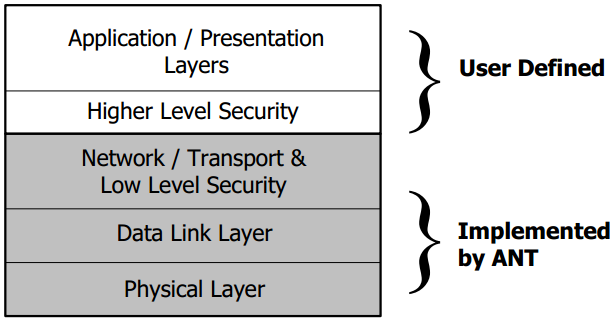
\includegraphics[scale=.5]{content/images/ANTstack.png}
	\caption{OSI-Layer vs. ANT Protocol\cite{Networks}}\label{fig:osilayer}
\end{figure}

This level of abstraction is achieved by incorporating the first 4 OSI-layers (see Figure \ref{fig:osilayer}) into the ANT protocol, thus allowing even low-cost microcontrollers to set up and maintain complex wireless networks, since all the details of the communication are handled by the ANT-chip.

\subsection{ANT Topology}
In order for the ANT protocol to work each mote needs to be part of a network. As shown in figure \ref{fig:anttopo} the ANT protocol can be used to create simple or considerably more complex networks. Each mote inside a network is called an ANT node. In order for two nodes to communicate with each other they need to be connected via a channel.

\begin{figure}[H]
	\centering
	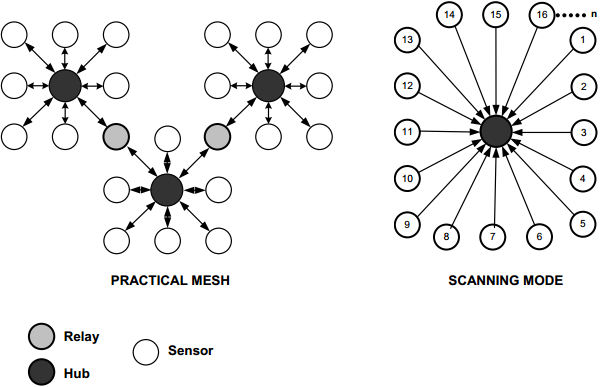
\includegraphics[scale=0.7]{content/images/ANTtopo.png}
	\caption{Example ANT Topologies\cite{DynastreamInnovationsInc.2013}}\label{fig:anttopo}
\end{figure}

\subsection{ANT Channels}
\label{sec:ANTchan}
The ANT protocol uses virtual channels to allow different nodes to transmit data. Each channel can be assigned to a 1 MHz wide RF frequency band between 2400 MHz and 2524 MHz.\cite{DynastreamInnovationsInc.2013} In theory this allows 125 different channels to exist without interference between them. It is possible for multiple channels to use the same frequency depending on the rate of transmission, since the data rate of each 1MHz band is limited to 1MBps. 
To avoid interference between nodes which use the same frequency isochronous self adjusting Time Division Multiple Access (TDMA) is used. TDMA allows the ANT protocol to adjust the transmit timings of the channels individually.

Each node has to specify how the assigned channel is being used. The node can either be a master or a slave node. While a master node mostly sends data and a slave node mostly receives data, the slave retains the ability to respond to the incoming data.

The ANT protocol further differentiates between two different channel types:
\begin{description}
	\item{\textbf{Independent Channels}} \hfill \\ Independent Channels are used if there is only one node which transmits data. There is no limit to the amount of slave devices which receive messages. Furthermore, the message being sent out is broadcast to all nodes. It is not possible to address only a specific node.
	
	\item{\textbf{Shared Channels}} \hfill \\ Shared Channels are used if there is more than one node which sends data. This type of channel is facilitated by the use of a Shared Channel Address, which in turn reduces the amount of data that can be transmitted at a time. All ANT nodes still receive every message, but only pass on messages which have a matching address. The Channel master can decide to either use one or two bytes as the address, which allows for either 255 or 65535 slave devices in the same channel. 
\end{description}

\begin{figure}[H]
	\centering
	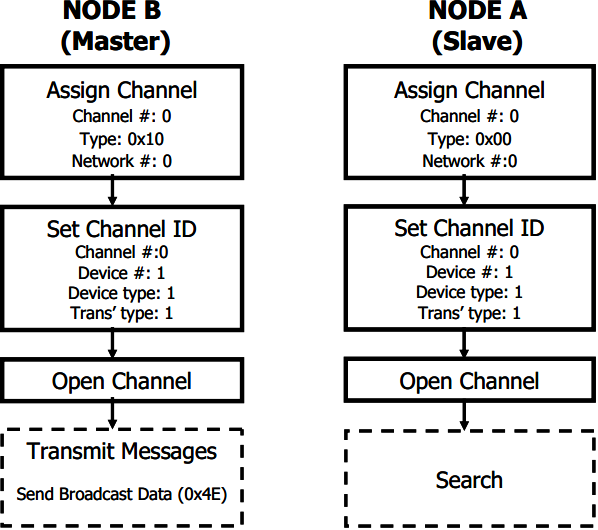
\includegraphics[scale=0.7]{content/images/ANTsetup.png}
	\caption{ANT channel establishment\cite{DynastreamInnovationsInc.2013}}\label{fig:antsetup}
\end{figure}

Figure \ref{fig:antsetup} shows the procedure of opening up a channel between two ANT nodes. In the first step the channel configuration is set, most important in this context being the channel type: 0x00 signifies that the node is opening the channel as a slave while 0x10 means that the node acts as a master. The next step is to set the Channel ID. Since it is possible for two nodes to transmit on the same frequency, the device number, device type and transmission type of the slave node need to match the values of the master it wants to connect to. It is possible, however, to set wild card values, which allows the slave to connect to any device sending on the same frequency. Before the final step, it is optionally possible to set the frequency of the channel, the power setting and the message period. These steps are not mandatory though, since ANT defaults to fixed values: 2466 Hz transmission frequency, 0dBm power and a message period of 8192. The last step constitutes of the opening of the channel itself. The master should open the channel before the slave to ensure a successful connection.

\subsection{ANT Communication}

The ANT protocol supports three different data types: broadcast, acknowledge and burst. The data type is not part of the channel configuration, thus channels are able to use any combination of data types. The only exceptions are legacy unidirectional channels, which can only send broadcast data. The various data types differ in the way data is handled and transmitted.
\begin{figure}[H]
	\centering
	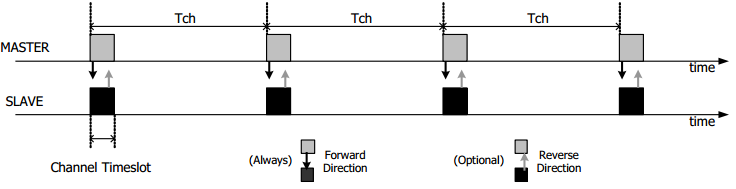
\includegraphics[scale=.75]{content/images/ANTdataflow.png}
	\caption{ANT channel communication \cite{DynastreamInnovationsInc.2013}}\label{fig:antflow}
\end{figure}

\begin{itemize}
	\item{Broadcast data} \hfill \\ Broadcast data represents the most basic data type and, at the same time, the default. To start a broadcast transmission, the command needs to be issued just once, since the last sent packet is continuously resent as a broadcast. It does not matter whether the last packet was part of a burst or acknowledge transmission. If no new data is available this packet is resent. Figure \ref{fig:antflow} shows, how each broadcast transmission is aligned to the channel with a message period $T_{ch}$. Since there is no answer from the receiving node, it is not possible to determine if the packet was transmitted correctly.
	
	\item{Acknowledge data} \hfill \\ Acknowledge data can be used to ensure a node has received a transmitted packet. After receiving an acknowledge packet the node will send a message back to the sender. Acknowledge data should only be used as a unicast, since if multiple nodes send an acknowledge message back, the messages can interfere with each other. Figure \ref{fig:antflow} shows that, just like broadcast data, acknowledge data is always aligned to a time slot, yet the receiver does not wait for the next time slot and instead sends the answer immediately back to the sender.
	
	\item{Burst data} \hfill \\ Burst data provides a method to quickly transmit larger amounts of data. This is achieved by ignoring the normal channel time slots and sending the packets immediately one after the other. This allows for a transmission rate of up to 20 kbps \cite{DynastreamInnovationsInc.2013}, which is much higher than the other data transmission types. Similar to acknowledge data, at the end of the transmission the sender is informed whether the transfer failed or succeeded. Just like acknowledge data, burst transmission should be unicast, since if one node fails to receive a packet the transmission is stopped. The drawback of this method is, that burst data is prioritized over all other transmissions and will interrupt other transmissions over the same RF frequency.
\end{itemize}

\subsection{ANT Messages}
In the ANT protocol each message has the basic format as specified in Figure \ref{fig:antmsg}.
\begin{figure}[H]
	\centering
	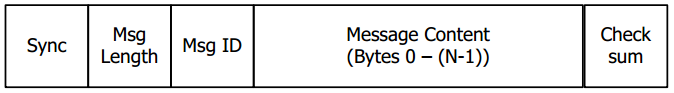
\includegraphics[scale=.75]{content/images/ANTmsg.png}
	\caption{ANT message structure\cite{DynastreamInnovationsInc.2013}}\label{fig:antmsg}
\end{figure}
Each message starts with a special Sync-Byte and ends with a checksum, which is calculated by xoring all previous bytes. The Msg Length byte shows the number of Message Content bytes. The Msg ID byte specifies which kind of data is contained in the message. The ANT protocol also provides an extended message format, which allows to attach further information to each message. The length of the message varies between message types, but the size of the payload for each of the three different data-transmission types is always at 8 bytes.

\section{ANT Library}
There is an official ANT library \cite{ANTWinLib} available, however this library is written in C++ for Windows. Since SHAMPU uses a PIC24FJ64GB002 microcontroller\cite{smeets2014demonstration} it is not possible to use the official library. Instead we use an already existing ANT library for this thesis \cite{ANTPICLIB}. This library implements almost the complete ANT API, except for two important features. The library uses busy-waiting to receive packets. Also sending burst transmission does not work correctly. In order to be able to use ANT efficiently with SHAMPU we implemented a non-blocking packet receiver. This is an important addition to the code, because otherwise the microcontroller is not able to function, while it is waiting for a packet. Unfortunately we were not able to get burst mode working correctly. Burst packets need to have a precise timing, but the black box nature of the ANT protocol makes it a challenge to debug the code.
\section{ANTAP1MxIB RF}
Each SHAMPU device is equipped with an ANTAP1MxIB RF Transceiver Module\cite{Networks}. The module was chosen because of its small form factor (20mm x 20mm) and its very low power draw. The ANTAP1M can handle up to 4 different ANT channels with a combined message rate of 200 Hz. 

\begin{figure}[H]
	\centering
	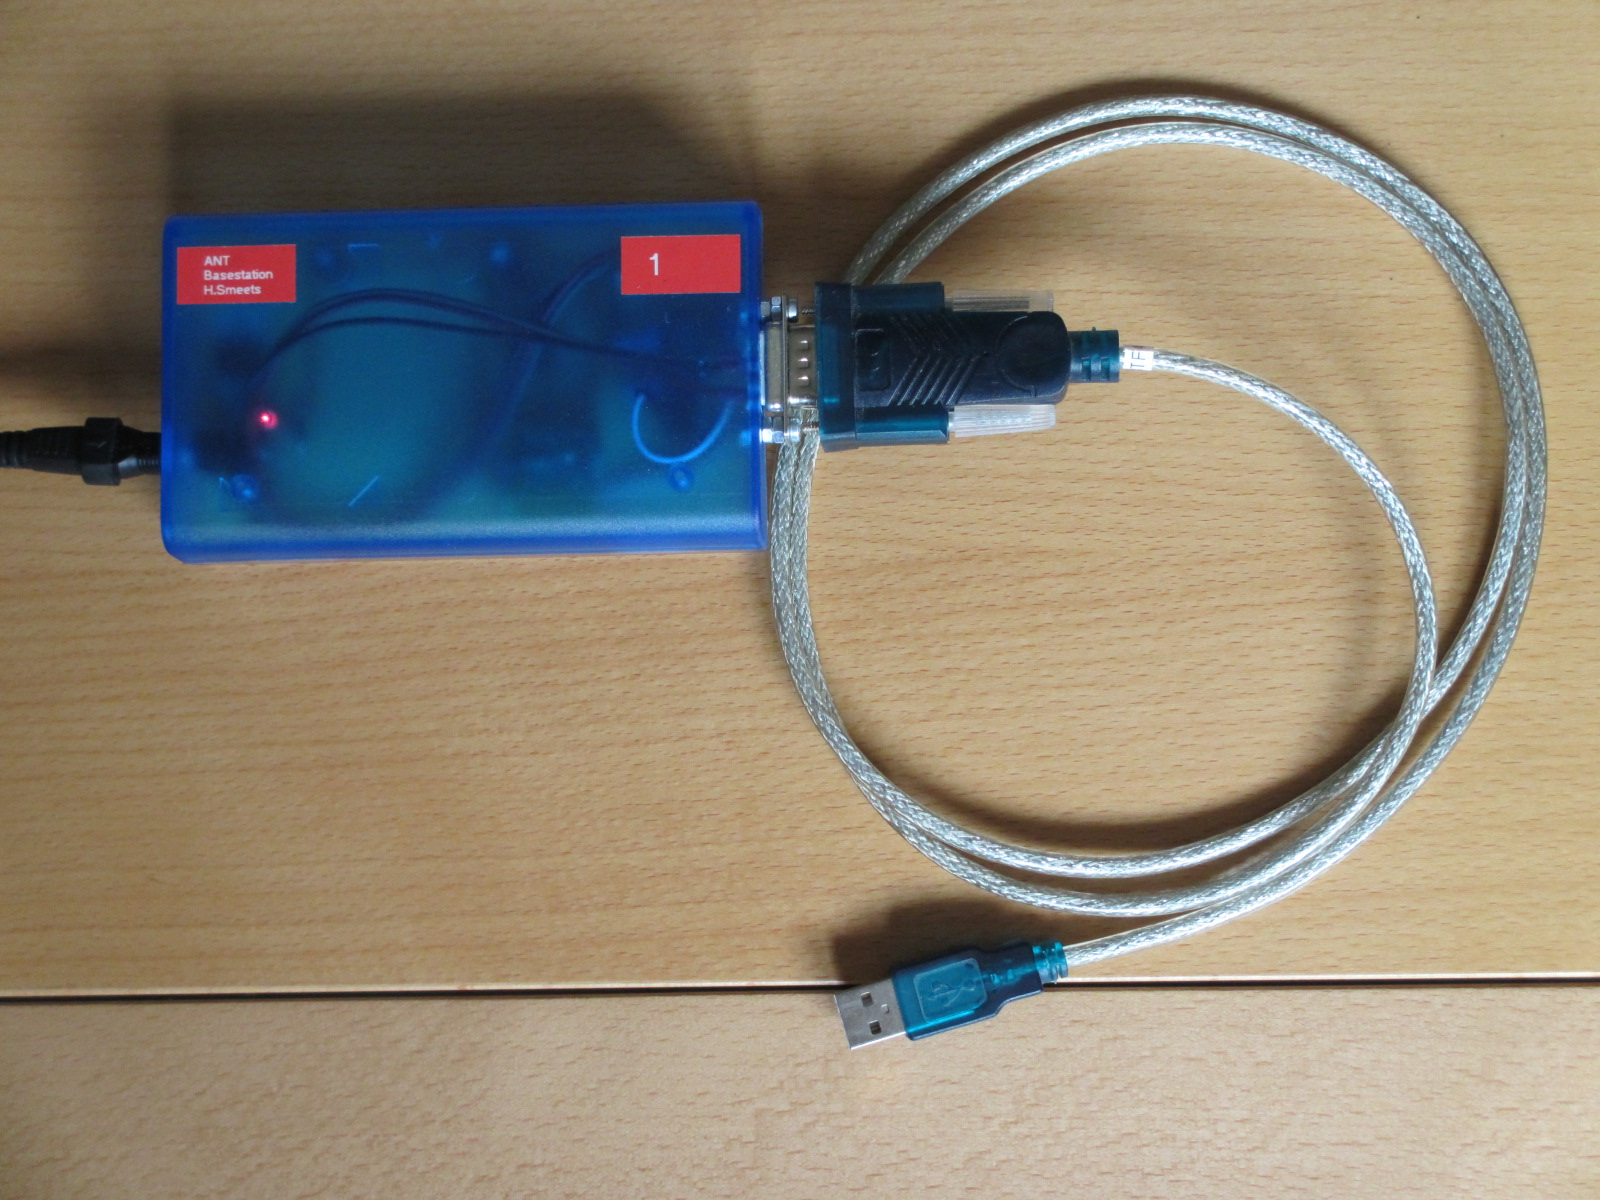
\includegraphics[scale=.5]{content/images/SHAMPUbase.JPG}
	\caption{SHAMPU base station}\label{fig:shampubase}
\end{figure}
In order to test the capabilities of the ANT chip, we used two SHAMPU base stations for all the experiments. This base station (see Figure \ref{fig:shampubase}) contains the ANTAP1MxIB and a MAX3224CPP microcontroller acting as an UART to serial interface, which allows the ANT to asynchronously communicate with a PC over RS-232. A transmission speed of 19200 baud is used which allows a data rate of 1920 Bps, since the RS-232 protocol adds a start and stop bit to each transmitted byte\cite{RS232}.
 %Technical Background

\chapter{Evaluation of SHAMPU}
In order to assess the capabilities of SHAMPU, we plan and run experiments designed to evaluate the SHAMPU framework according to the following use-cases:
\begin{itemize}
	\item{\textbf{Scheduled data-transmission}} \hfill \\ In order for SHAMPU to work as a debugging and logging platform, the base station needs to periodically receive data from all the nodes in the network. Furthermore the base station has to be able to send commands to nodes in the network.
	\item{\textbf{Unscheduled data-transmission}} \hfill \\ There are several cases, where it is not feasible to use a scheduled data-transmission. Because either the data only needs to be transmitted once, or it is not know at what point in time the transmission happens: 
	\begin{itemize}
		\item{}Reprogramming of a node: SHAMPU is able to reprogram the attached node. For this process, SHAMPU needs to receive a new firmware, which can amount to several hundred kB.
		\item{}SHAMPU RAM-Dumps: SHAMPU has 128kB of RAM, which can be used to save collected data during an experiment. At the end of the experiment the complete memory needs to be transmitted back to the base station.
	\end{itemize}
\end{itemize}
	
To evaluate ANT according to these two use-cases, we identified three metrics which indicate how well a use-case can be handled:
	\begin{itemize}
		\item {\textbf{Data throughput }} \hfill \\ The speed with which ANT can transmit data directly affects the network performance and how many nodes can be part of the network at once. ANT provides three different data types which can be used to transport data: Broadcast data and acknowledge data can be used for scheduled data-transmission. Burst mode can be used for unscheduled data-transmission. 		
		
		\item {\textbf{Message delay}} \hfill \\ A SHAMPU base station not only acts as a data sink for incoming logging information, but is also able to send commands to other SHAMPU devices in the network.
		It is thus important to know how long it takes ANT to verify whether a message was correctly received or not.
		
		\item {\textbf{Communication range}} \hfill \\ Since SHAMPU is architecture independent it can be used in different situations. Therefore it is important to know, how far away from the base station the nodes can be placed. As SHAMPU focuses on energy efficiency, it might also be viable to reduce the range for smaller set ups to save even more energy.
	\end{itemize}

To cover the mentioned metrics we designed different experiments, which test one or more of the described categories. The following section describes the experiments according to the following template:

\begin{description}
	\item{\textbf{Description}} \hfill \\ A description of the experiment and the category being evaluated.
	\item{\textbf{Use-Case}} \hfill \\ The use-case which the experiment tries to test.
	\item{\textbf{Network topology and pseudo code}} \hfill \\ A diagram of the network topology in which the experiment is run and pseudo code which describes the program being run on the master and the slave. Missing values are default values and described in section \ref{sec:commonPara}.
	\item{\textbf{Testing methodology}} \hfill \\ A description how the experiment is performed.
	\item{\textbf{Result}} \hfill \\ The results of the experiment and any additional data collected during the experiment.
\end{description}

\newpage

\section{Common experiment parameters}
\label{sec:commonPara}
\begin{figure}[H]
	\centering
	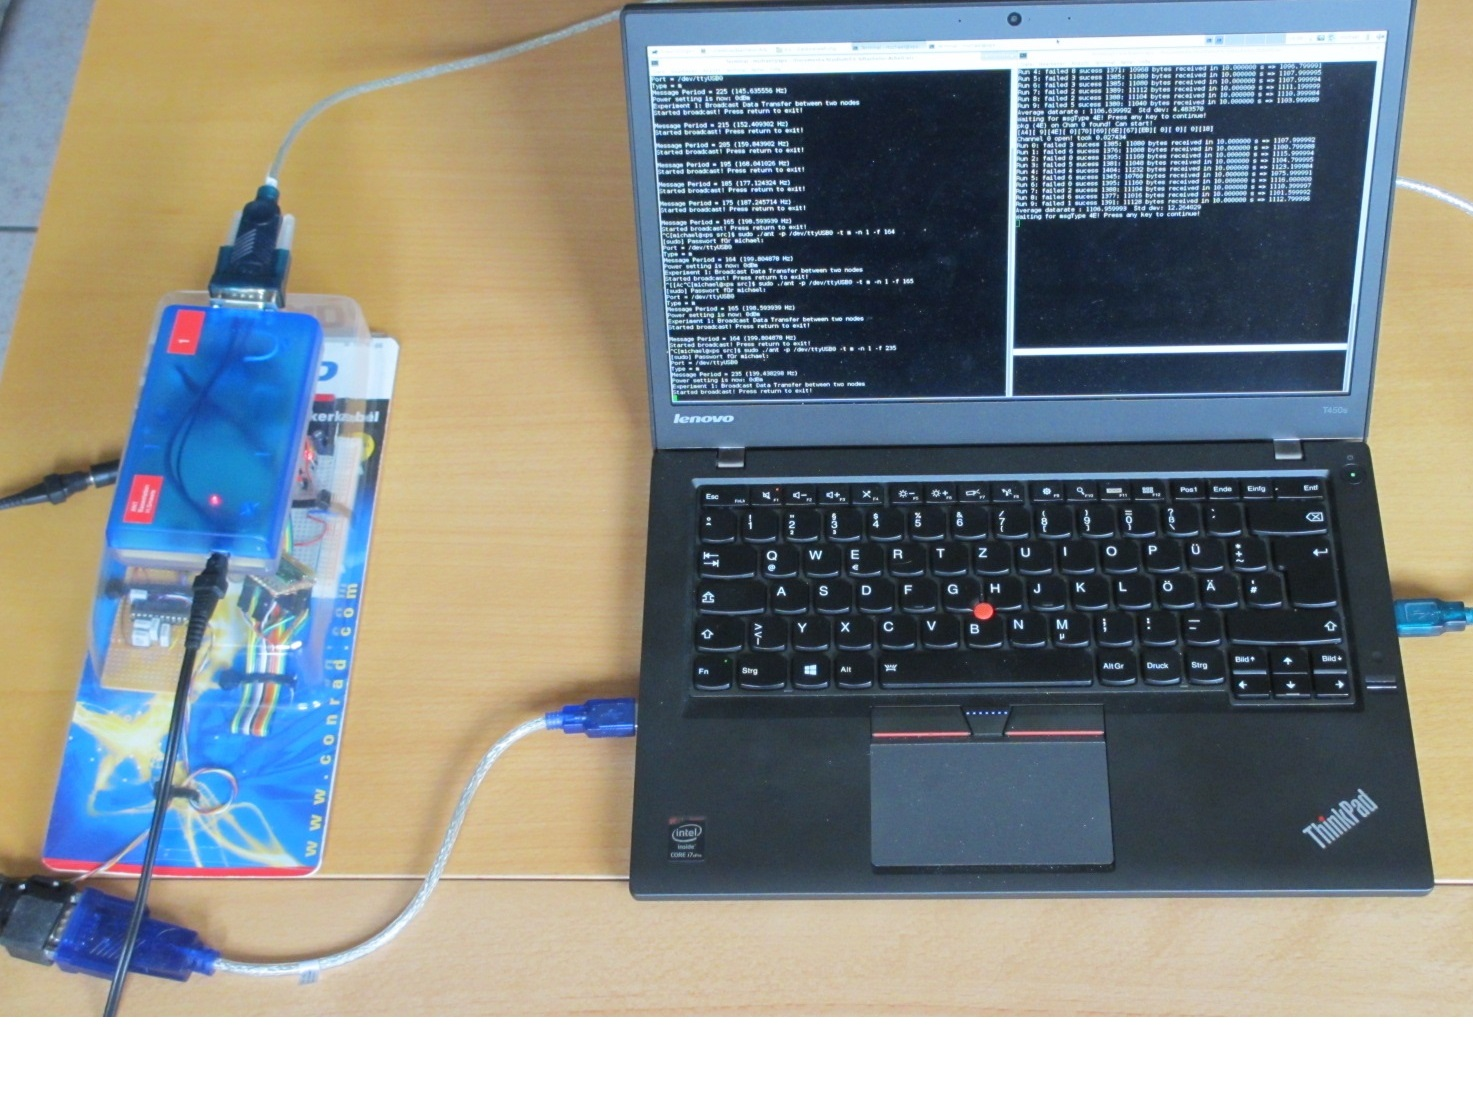
\includegraphics[scale=.75]{content/images/expSetup.JPG}
	\caption{Experiment set up}\label{fig:expSetup}
\end{figure}

If not otherwise noted in the description each experiment was run in the Mobility Lab of the Networked Embedded Systems group at the University of Duisburg-Essen (SA 327), with the two base stations in the configuration which can be seen in figure \ref{fig:expSetup}. The following table describes the parameters which were used in the experiments.

\begin{table}[H]
	\centering
	\begin{tabular}{|l|c|c|}
		\hline
		Device number        & 33    & \multirow{3}{*}{\begin{tabular}[c]{@{}c@{}}Channel ID\\ (see section \ref{sec:ANTchan})\end{tabular}}   \\ \cline{1-2}
		Device type          & 1     &                                                                                                         \\ \cline{1-2}
		Transmission type    & 1     &                                                                                                         \\ \hline
		ID\_CHAN1            & 0     & \multirow{2}{*}{\begin{tabular}[c]{@{}c@{}}Configuration\\ for the first channel\end{tabular}}          \\ \cline{1-2}
		FREQ\_CHAN1          & 66 Hz &                                                                                                         \\ \hline
		ID\_CHAN2            & 1     & \multirow{2}{*}{\begin{tabular}[c]{@{}c@{}}Configuration\\ for the second channel\end{tabular}}         \\ \cline{1-2}
		FREQ\_CHAN2          & 77 Hz &                                                                                                         \\ \hline
		STD\_FREQ            & 8192  & 4 Hz (default frequency)                                                                                \\ \hline
		min\_Channel\_Period & 164   & 199.8 Hz (closest to 200 Hz)                                                                            \\ \hline
		max\_Channel\_Period & 65535 & 0.5 Hz (smallest frequency)                                                                             \\ \hline
		STD\_POWER           & 0 dBm & 1 mW (default transmit power)                                                                           \\ \hline
	\end{tabular}
	\caption{ANT default configuration}
\end{table}

There is an important difference between the message period used in the pseudo code and the frequency used in the figures which display the results. The period describes the size of the gap between two messages, the frequency describes how many messages are sent in 1 second. The channel period $p$ can be used to calculate the frequency of the messages $f_t = \frac{32678s^{-1}}{p}$. For example a message period of 8192 results in a message frequency of 4 Hz, which means that 4 messages are send every second.

ANT supports different transmit power levels: 0 dBm, -5 dBm, -10 dBm and -20 dBm. dBm is a way to express broadcast power as a power ratio in decibels. The power of the broadcast $p$ can be calulated as follows $p = 1mW * 10^{\frac{x}{10}}$.

Furthermore in experiments which measure data throughput, we show maximum theoretical value for each frequency. This is the maximum value which can be achieved, if there are no transmission errors and no interference with other channels. The value depends on the message frequency $f$ and be calculated as follows: $rate_{max}(f) = 8*f$. Each message contains contains a payload of 8 bytes and we send $f$ messages each second.
\newpage

\section{Experiment 1: Broadcast Data Transfer between two nodes}
\begin{description} 
	\item{\textbf{Description}} \hfill \\ Broadcasting is one way of periodically transmitting data between two or more ANT nodes. Since all broadcast packets are synchronized to a fixed time-slot, the data throughput can be increased by decreasing the channel period. The experiment itself is split into two parts. In the first part we try to determine the highest possible data throughput. Also we try to determine whether the channel period has an effect on the time it takes for a slave node to find and join an existing channel. The second part is a test of the highest detected data throughput. Here we try to evaluate if there are any variations of the data throughput over a much longer interval.	
	\item{\textbf{Use-Case}} \hfill \\ Scheduled data-transmission	
	\item{\textbf{Network topology and pseudo code}} \hfill \\ 
	\begin{figure}[H]
		\centering
		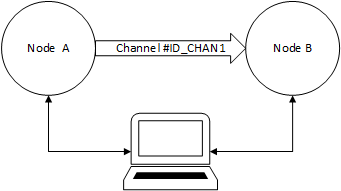
\includegraphics[scale=1]{content/images/exp_topo.png}
		\caption{Topology experiment 1}
	\end{figure}
	\begin{code}[H]
		\begin{verbatim}
		channelPeriod = max_Channel_Period
		while (channelPeriod >= min_Channel_Period)
		  ANT_SetChannelPeriod(ID_CHAN1, channelPeriod)
		  ANT_OpenChannel(ID_CHAN1, ANT_Bidirectional_Master)
		  ANT_SendBroadcastData(ID_CHAN1, [0x01, 0x02, 0x03, 0x04])
		  wait_for_user_input()
		  ANT_CloseChannel(ID_CHAN1)
		  if (channelPeriod >= 0x00FF)
		    channelPeriod = channelPeriod >> 1
		  else
		    channelPeriod = channelPeriod - 10
		\end{verbatim}
		\caption{Broadcast data single channel (Master)}\label{lst:mExp1}
	\end{code}
	
	\begin{code}[H]
		\begin{verbatim}
		channelPeriod = max_Channel_Period
		while (channelPeriod >= min_Channel_Period) 
		  for (i in 0..10) 
		    ANT_SetChannelPeriod(ID_CHAN1, channelPeriod)
		    ANT_OpenChannel(ID_CHAN1, ANT_Bidirectional_Slave)
		    count = 0
		    for (100 seconds) 
		      if (receivedPacket() == ANT_BROADCAST_DATA)
		        count++;			  
		    print (count * 8 / 100) + " Bytes per second"
		    wait_for_user_input()
		    ANT_CloseChannel(ID_CHAN1)
		  if (channelPeriod >= 0x00FF)
		    channelPeriod = channelPeriod >> 1
		  else
		    channelPeriod = channelPeriod - 10
		\end{verbatim}
		\caption{Broadcast data single channel (Slave)}\label{lst:sExp1}
	\end{code}	
	\item{\textbf{Testing methodology}} \hfill \\Experiment 1 is split into two parts.
	In the first part node A acts as the master and node B as the slave. For both nodes the channel period is set to the highest value and the channel is opened. Node B records how long it takes to join the channel and how many bytes it receives over a 100s interval. The measurement is repeated 10 times and the average values are saved. Then the channel period is decreased and the process is repeated.\\ 
	In the second part of the experiment, the channel period is set to the value which achieved the highest speed. The experiment is then left running for a period of 10 hours and the data throughput is recorded in one continuous run.
	\item{\textbf{Result}} \hfill \\  
	\begin{figure}[H]
		\centering
		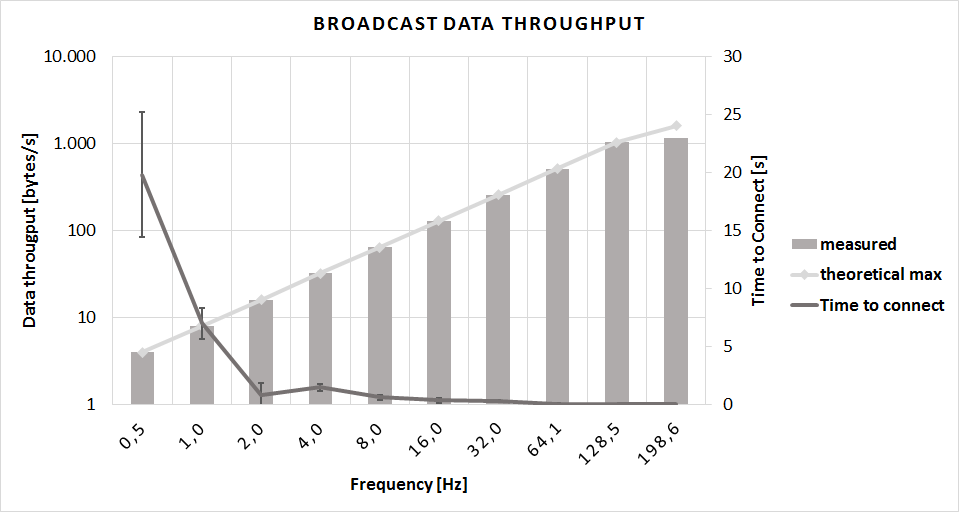
\includegraphics[scale=0.5]{content/images/exp1_norm.png}
		\caption{Broadcast data rate (0.5Hz - 198.6Hz)}\label{fig:exp1norm}
	\end{figure}
	
	Figure \ref{fig:exp1norm} shows the transmission speeds achieved for the different frequencies. Up to a frequency of 128 Hz, the measured data rate matches the expected theoretical maximum rate. For the highest measured frequency (198.6 Hz), the data rate is much lower than the maximum rate. The measured errors are insignificant. Therefore the frequencies between 128 Hz and 198.6 Hz were analyzed in more detail. 
		
	The time it takes for a Node to join a channel falls rapidly once the frequency is above 1 Hz. For frequencies above 64 Hz, the time it takes to join a channel becomes negligible, with times around 75 ms (see Figure \ref{fig:exp1norm}). All the measured values are below the specified worst case channel acquisition times of the ANT protocol \cite{AntChan}.
	
	\begin{figure}[H]
		\centering
		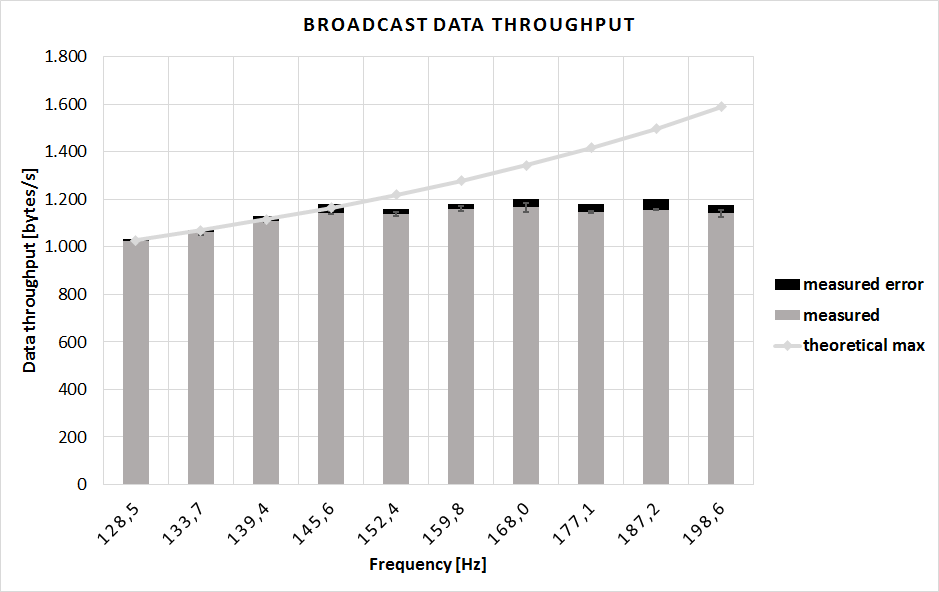
\includegraphics[scale=0.5]{content/images/exp1_detail.png}
		\caption{Broadcast data rate (129Hz - 198.6Hz)}\label{fig:exp1between}
	\end{figure}
	As seen in figure \ref{fig:exp1between} the measured data rates for frequencies above 140 Hz all fall short of the expected values. The average data throughput of these frequencies remains consistently at around 1100 Bps. The experiment was repeated multiple times, running it at different times and places, thus an environmental factor can be excluded. That means, the reason for the upper limit has to be found with the test set up itself. See section \ref{sec:dataThrougput} for a discussion about possible reasons for this upper limit.
	
	\begin{figure}[H]
		\centering
		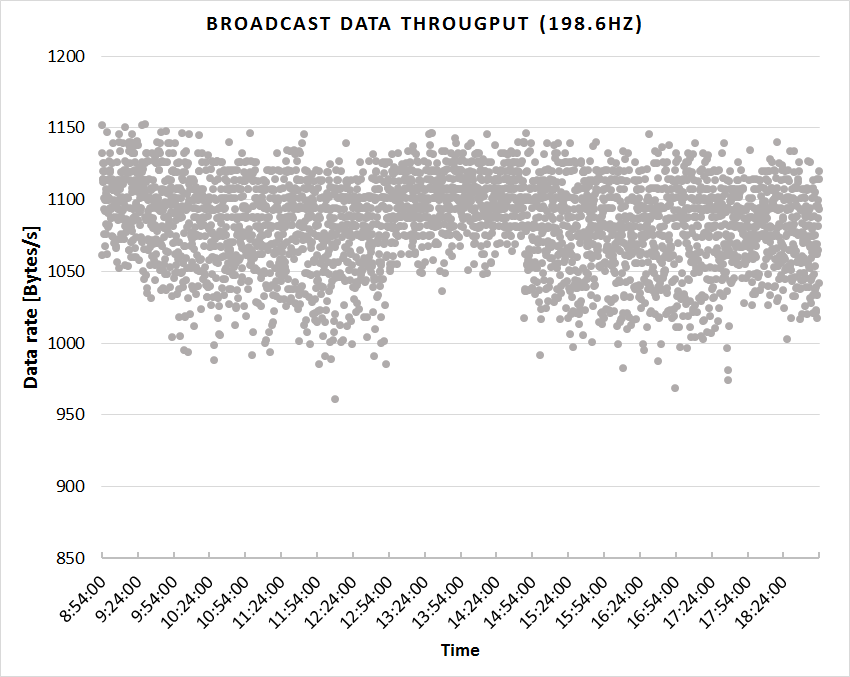
\includegraphics[scale=0.5]{content/images/exp1_long.png}
		\caption{Broadcast data rate over time (198.6Hz)}\label{fig:exp1long}
	\end{figure}
	Figure \ref{fig:exp1long} shows the transmission speed for the highest supported frequency 198.6 Hz over time. The results show that the data throughput stays fairly consistent at around 1100 Bps with a standard deviation of only 30 Bps, or 2.7\%. Interesting to note is the time period from 1:00PM to 2:50 PM, where the deviation from the average is much smaller. The exact reason for this phenomenon in unknown, since during this time period the environment of the test set up did not change in any known way.
\end{description}
\newpage

\section{Experiment 2: Broadcast Data Transfer with two channels}
\begin{description} 
	\item{\textbf{Description}} \hfill \\ In experiment 1 we determined the channel period, which allows for the maximum throughput. In this experiment we try to determine, how the maximum throughput is affected by the amount of channels in the network. SHAMPU needs two channels, so it can work correctly: One channel which sends data from the base station to the nodes in order to control them and another channel by which the nodes can send debugging and other information.
	\item{\textbf{Use-Case}} \hfill \\ Scheduled data-transmission	
	\item{\textbf{Network topology and pseudo code}} \hfill
	\begin{figure}[H]
		\centering
		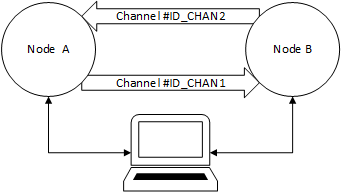
\includegraphics[scale=1]{content/images/exp2_topo.png}
		\caption{Topology experiment 2}
	\end{figure}
	\begin{code}[H]
		\begin{verbatim}
		channelPeriod = max_Channel_Period
		while (channelPeriod >= min_Channel_Period) 
		  ANT_SetChannelPeriod(ID_CHAN1, channelPeriod)
		  openChannel(ID_CHAN1, ANT_Bidirectional_Master)
		  ANT_SendBroadcastData(ID_CHAN1, [0x01, 0x02, 0x03, 0x04])
		  ANT_SetChannelPeriod(ID_CHAN2, channelPeriod)
		  openChannel(ID_CHAN2, ANT_Bidirectional_Slave)
		  count = 0
		  for (100 seconds) 
		    if (receivedPacket() == ANT_BROADCAST_DATA)
		      count++			
		  print (count * 8 / 10) + " Bytes per second"
		  wait_for_user_input()
		  ANT_CloseChannel(ID_CHAN1)
		  ANT_CloseChannel(ID_CHAN2)
		  if (channelPeriod >= 0x01FF)
		    channelPeriod = channelPeriod >> 1
		  else
		    channelPeriod = channelPeriod - 10
		 \end{verbatim}
		\caption{Broadcast data transfer two channels (Master)}\label{lst:mExp2}
	\end{code}
	
	\begin{code}[H]
		\begin{verbatim}
		channelPeriod = max_Channel_Period
		while (channelPeriod >= min_Channel_Period)
		  ANT_SetChannelPeriod(ID_CHAN1, channelPeriod)
		  openChannel(ID_CHAN1, ANT_Bidirectional_Slave)
		  ANT_SetChannelPeriod(ID_CHAN2, channelPeriod)
		  openChannel(ID_CHAN2, ANT_Bidirectional_Master)
		  ANT_SendBroadcastData(ID_CHAN2, [0x01, 0x02, 0x03, 0x04])
		  count = 0
		  for (100 seconds) 
		    if (receivedPacket() == ANT_BROADCAST_DATA)
		      count++			
		  print (count * 8 / 10) + " Bytes per second"
		  wait_for_user_input()
		  ANT_CloseChannel(ID_CHAN1)
		  ANT_CloseChannel(ID_CHAN2)
		  if (channelPeriod >= 0x01FF)
		    channelPeriod = channelPeriod >> 1
		  else
		    channelPeriod = channelPeriod - 10
		\end{verbatim}
		\caption{Broadcast data transfer two channels (Slave)}\label{lst:mExp2}
	\end{code}
	
	\item{\textbf{Network topology and pseudo code}} \hfill \\ The two nodes are placed right next to each other.
	
	\item{\textbf{Testing methodology}} \hfill \\ In this experiment each node acts as a master for a different channel. Node A is the master for Channel 0 and Node B is the master for Channel 1. The measurements themselves are identical to the ones in experiment 1, except that the data is recorded on both nodes. The channel period is then decreased until the data throughput no longer increases, or the connections breaks completely.
	
	\item{\textbf{Result}} \hfill \\  	
	\begin{figure}[H]
		\centering
		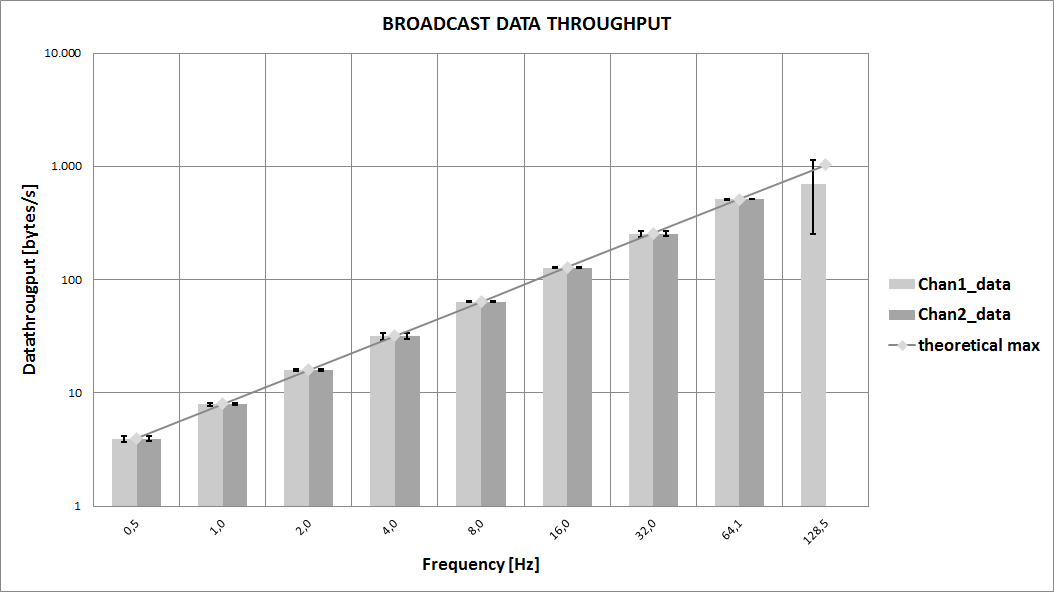
\includegraphics[scale=0.5]{content/images/exp2_norm.png}
		\caption{Broadcast data through - 2 channels (0.5Hz - 129Hz)}\label{fig:exp2low}
	\end{figure}
	Figures \ref{fig:exp2low} shows the results of the measurements, the left bar displaying the throughput for channel 1, the right bar displaying the throughput for channel 2. Just as in experiment 1 the  line shows the theoretical maximum of the data throughput for the given frequency. Up to a frequency of 64 Hz the data throughput increases with the frequency for both channels and matches the maximum value very closely. However the data throughput of channel 2  drops to zero at 128 Hz, while the data throughput of channel 1 almost matches the expected value.
		\begin{figure}[H]
			\centering
			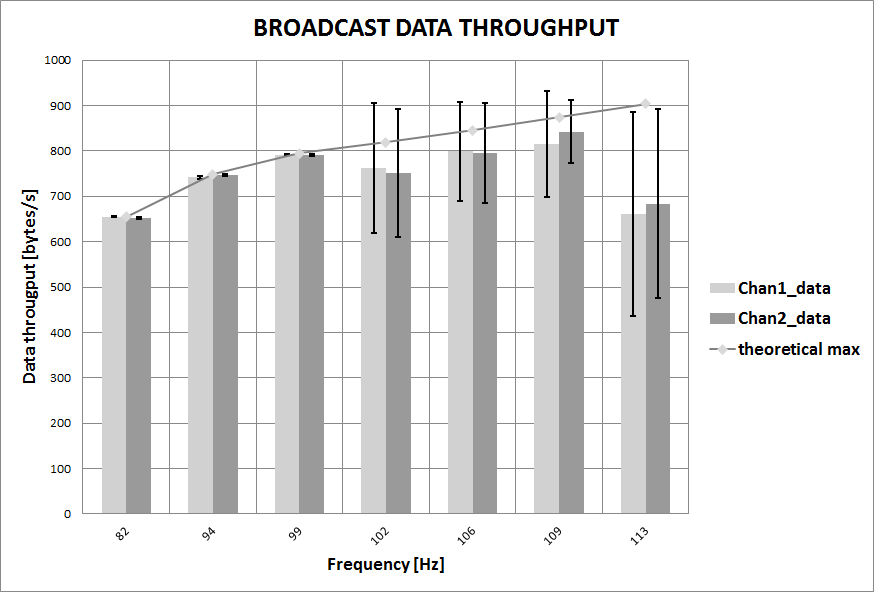
\includegraphics[scale=0.5]{content/images/exp2_detail.png}
			\caption{Broadcast data through - 2 channels (64Hz - 129Hz)}\label{fig:exp2high}
		\end{figure}
	To further investigate this drop off, figure \ref{fig:exp2high} shows the data throughput for chosen frequencies between 82 Hz and 113 Hz. The figure clearly shows that somewhere between 82 Hz and 99 Hz the data throughput matches the expect values. For frequencies over 100 Hz however the data throughput begins to drop off, while the measured error increases. From this result we conclude two things: The 200 Hz combined rate of the ANT chip is split between all channels the chip joined. In this case each chip broadcasts with 100 Hz and receives with 100 Hz, resulting in a data throughput of around 800 Bps for each channel. See section \ref{sec:dataThrougput} for a discussion about this upper limit. 	
	
\end{description}
\newpage


\section{Experiment 3: Acknowledge Data Transfer between two nodes}
\begin{description} 
	\item{\textbf{Description}} \hfill \\ This experiment is almost identical with experiment 1. The main difference is that we use acknowledge data instead of broadcast. It is also important to note that the master records how many successful packets are transmitted. The main goal of the experiment is to see whether the data throughput is decreased compared to broadcast data, especially for smaller channel periods.
	\item{\textbf{Use-Case}} \hfill \\ Scheduled data-transmission
	\item{\textbf{Network topology and pseudo code}} \hfill \\
	\begin{figure}[H]
		\centering
		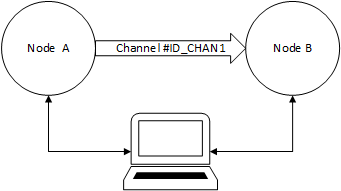
\includegraphics[scale=1]{content/images/exp_topo.png}
		\caption{Topology experiment 3}
	\end{figure}
	\begin{code}[H]
		\begin{verbatim}
		channelPeriod = max_Channel_Period
		while (channelPeriod >= min_Channel_Period) 
		  ANT_SetChannelPeriod(ID_CHAN1, channelPeriod)
		  ANT_OpenChannel(ID_CHAN1, ANT_Bidirectional_Master)
		  count = 0
		  for (10 seconds) 
		    ANT_SendAcknowledgedData(ID_CHAN1, [0x01, 0x02, 0x03, 0x04])	   
		    wait_for_ack()
		    count++
		  print (count * 8 / 10) + " Bytes per second"	  
		  ANT_CloseChannel(ID_CHAN1)
		  if (channelPeriod >= 0x00FF)
		    channelPeriod = channelPeriod >> 1
		  else
		    channelPeriod = channelPeriod - 10
		\end{verbatim}
		\caption{Acknowledge data transfer (Master)}\label{lst:mExp3}
	\end{code}
	
	\begin{code}[H]
		\begin{verbatim}
		channelPeriod = max_Channel_Period
		while (channelPeriod >= min_Channel_Period) 
		  ANT_SetChannelPeriod(ID_CHAN1, channelPeriod)
		  ANT_OpenChannel(ID_CHAN1, ANT_Bidirectional_Slave)
		  wait_for_user_input()
		  ANT_CloseChannel(ID_CHAN1)
		  if (channelPeriod >= 0x00FF)
		    channelPeriod = channelPeriod >> 1
		  else
		    channelPeriod = channelPeriod - 10
		\end{verbatim}
		\caption{Acknowledge data transfer (Slave)}\label{lst:sExp3}
	\end{code}
	\item{\textbf{Testing methodology}} \hfill \\ The testing methodology is the same as experiment 1, except that the master sends acknowledge messages and waits for the slave to confirm the successful transmission before sending the next packet. 
	\newpage
	\item{\textbf{Result}} \hfill \\
	\begin{figure}[H]
		\centering
		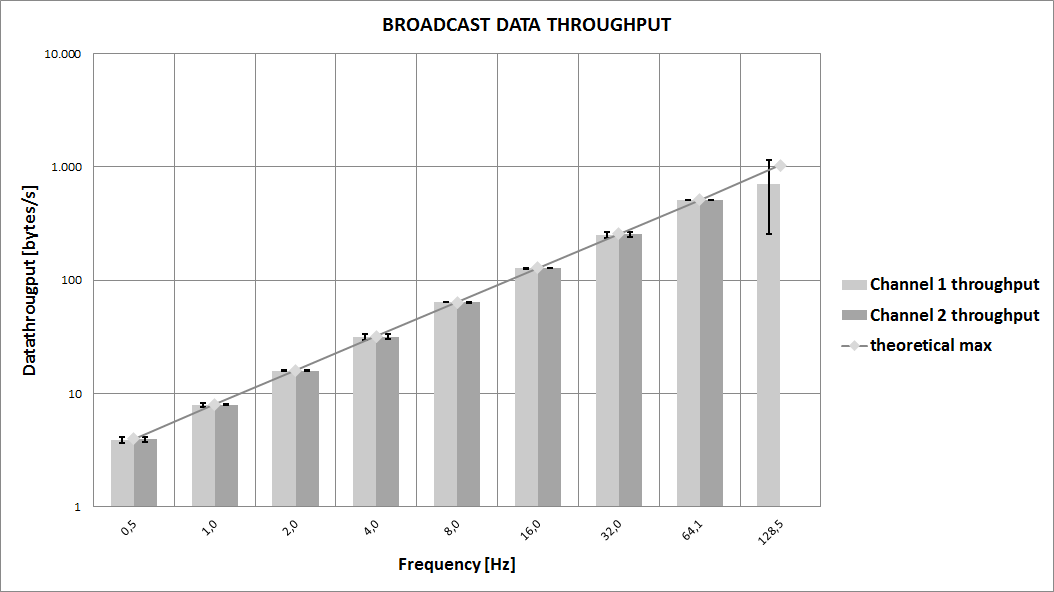
\includegraphics[scale=0.5]{content/images/exp3_norm.png}
		\caption{Acknowledge data rate (0.5Hz - 129Hz)}\label{fig:exp4norm}
	\end{figure}
	\begin{figure}[H]
		\centering
		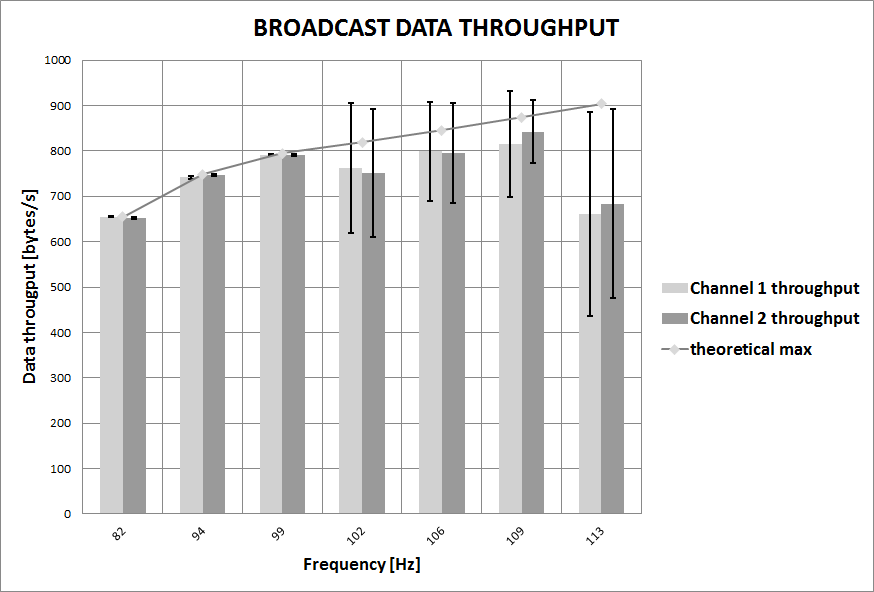
\includegraphics[scale=0.5]{content/images/exp3_detail.png}
		\caption{Acknowledge data rate (65Hz - 70Hz)}\label{fig:exp4between}
	\end{figure}
	
	Figure \ref{fig:exp4norm} shows the measured transmission speeds for the different tested frequencies. For the lower frequencies, the values align very well with the maximum data rate. Notable however is the drop off at 129 Hz. Figure \ref{fig:exp4between} shows the data throughput for some chosen values, between 64 Hz and 129 Hz. Demonstrating that the drop off starts around 69 Hz. 
	
	We conclude that the data throughput is a result of ANT retransmitting the last sent packet as broadcast data. If the frequency for this retransmission is too high it can interfere with the acknowledge message that the slave sends back to the master. For example at 128 Hz the message is broadcast every ~7 ms, resulting in too much data for the channel to handle. The transmission is thus interrupted. 
	Since there is no increase of the data throughput between 64 Hz and 128 Hz, but a huge drop off at 69 Hz it can be assumed that somewhere around 69 Hz the channel is at the maximum data throughput of around 1100 Bps. Again see section \ref{sec:dataThrougput} for a discussion about possible reasons for this upper limit. 	
\end{description}
\newpage

\section{Experiment 4: Acknowledge Transfer delay}
\begin{description} 
	\item{\textbf{Description}} \hfill \\ In this experiment we try to determine the time it takes for a node to receive and acknowledge a transmitted packet. The value is important in order to be able to determine the reaction time of SHAMPU to commands sent by the base station, for example to set up a separate channel for a burst transmission.
	\item{\textbf{Use-Case}} \hfill \\ Scheduled data-transmission
	\item{\textbf{Network topology and pseudo code}} \hfill \\ 
	\begin{figure}[H]
		\centering
		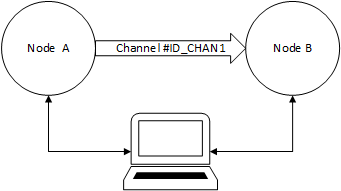
\includegraphics[scale=1]{content/images/exp_topo.png}
		\caption{Topology experiment 4}
	\end{figure}
	\begin{code}[H]
		\begin{verbatim}
		channelPeriod = max_Channel_Period
		while (channelPeriod >= min_Channel_Period) {
		  ANT_SetChannelPeriod(ID_CHAN1, channelPeriod);
		  ANT_OpenChannel(ID_CHAN1, ANT_Bidirectional_Master);
		  duration = 0.0
		  for (i in 0..10) {
		    ANT_SendAcknowledgedData(ID_CHAN1, [0x01, 0x02, 0x03, 0x04])
		    start = getTime()	   
		    wait_for_ack()		
		    print (getTime() - start) + " s"	  
		  ANT_CloseChannel(ID_CHAN1)		
		  if (channelPeriod >= 0x00FF)
		    channelPeriod = channelPeriod >> 1
		  else
		    channelPeriod = channelPeriod - 10
		\end{verbatim}
		\caption{Acknowledge data delay (Master)}\label{lst:mExp4}
	\end{code}
	
	\begin{code}[H]
		\begin{verbatim}
		channelPeriod = max_Channel_Period
		while (channelPeriod >= min_Channel_Period)
		  ANT_SetChannelPeriod(ID_CHAN1, channelPeriod);
		  ANT_OpenChannel(ID_CHAN1, ANT_Bidirectional_Slave);				 
		  wait_for_user_input();
		  ANT_CloseChannel(ID_CHAN1);
		  if (channelPeriod >= 0x00FF)
		    channelPeriod = channelPeriod >> 1
		  else
		    channelPeriod = channelPeriod - 10
		\end{verbatim}
		\caption{Acknowledge data delay (Slave)}\label{lst:sExp4}
	\end{code}
	
	\item{\textbf{Testing methodology}} \hfill \\ Node A acts as the master and node B as the slave. For both nodes the channel period is set to the highest value and the channel is opened. Node A then sends a total of 10 acknowledge messages and measures how long it takes until it receives the
	acknowledge signal. The channel period is then decreased and the experiment repeated.
	
	\newpage
	\item{\textbf{Result}} \hfill \\  
	\begin{figure}[H]
		\centering
		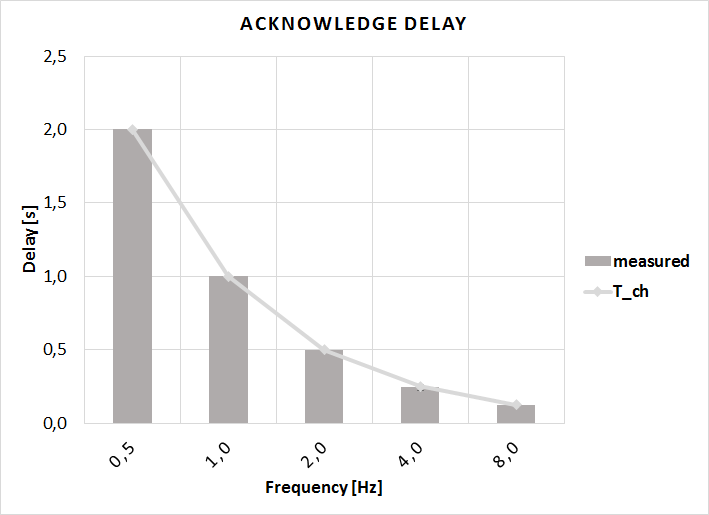
\includegraphics[scale=0.5]{content/images/exp4_norm.png}
		\caption{Acknowledge delay (0.5Hz - 8Hz)}\label{fig:exp3low}
	\end{figure}
	\begin{figure}[H]
		\centering
		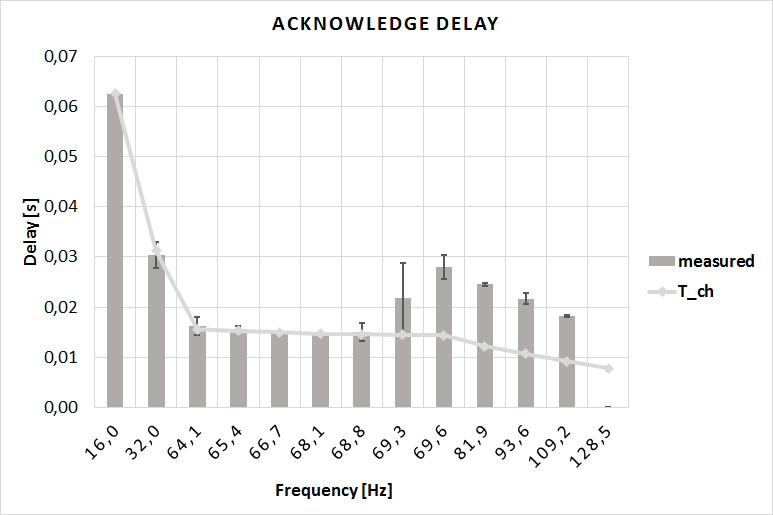
\includegraphics[scale=0.5]{content/images/exp4_detail.png}
		\caption{Acknowledge delay (16Hz - 70Hz)}\label{fig:exp3high}
	\end{figure}
	Figure \ref{fig:exp3low} and \ref{fig:exp3high} show the delays for the tested frequencies. The line shows the size of the gap between two timeslots and can act as a resolution for each measurement. For the lower frequencies the results are skewed, since each acknowledge packet is aligned to a time-slot. Thus, since ANT waits to send the acknowledge message the biggest part of the delay is waiting for the next time-slot. For frequencies greater than 64 Hz and below 68.8 Hz the data is considerably more useful, since the gap between two time-slots is lower than the measured values. The delay for those frequencies is around 18 ms, with no notable difference between 128 Hz and 200 Hz. Since the reply is always send directly after the message arrived, it can be assumed that the delay for the higher channel periods is the same as the one for the lower channel periods.
	
	The increase in the delay time for frequencies 68.8 Hz and greater can be explained with the results from experiment 3, where we determined that above 68 Hz the data throughput decreases. Since it is not possible to receive and send a package at the same time, the acknowledge message has to wait before it can be sent.
\end{description}
\newpage

\section{Experiment 5: Burst Data Transfer between two nodes}
\begin{description} 
	\item{\textbf{Description}} \hfill \\ Burst data transmissions make it possible to drastically increase the throughput rate. This allows a SHAMPU base station to quickly transmit a new firmware to a node or a node to dump its RAM back to the base station.	According to the  specification rates of up to 20 kbps can be achieved. To fully utilize this speed a baud rate of 50000 is needed. In the current set up the base station uses 19200 baud, since it is the only value that both the ANT chip and the RS-232 Interface support. Because of this we expect the maximum speed to be less than 20 kbps. Furthermore we try to determine whether the size of the burst transfer has an impact on the speed, since longer bursts will disrupt communications on other channels.
	\item{\textbf{Use-Case}} \hfill \\ Unscheduled data-transmission
	\item{\textbf{Network topology and pseudo code}} \hfill \\ 
	\begin{figure}[H]
		\centering
		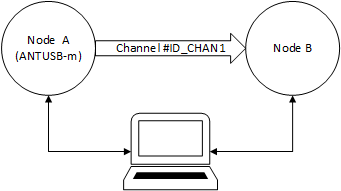
\includegraphics[scale=1]{content/images/exp5_topo.png}
		\caption{Topology experiment 5}
	\end{figure}
	\begin{code}[H]
		\begin{verbatim}
		size = START_SIZE
		ANT_OpenChannel(ID_CHAN1, ANT_Bidirectional_Slave);		
		while (size >= END_SIZE)
		  for (i in 0..10) 
		    // The first packet of a burst has the 3 MSB of the channelID field set to 0
		    wait_until(received_Packet == ANT_BURST_DATA && 
		               (received_message_channelID[0] & 0xE0) == 0x00)
		    start = getTime()
		    // The last packet of a burst has the MSB of the channelID field set to 1
		    wait_until(received_Packet == ANT_BURST_DATA && 
		               (received_message_channelID[0] & 0x80) > 0)		    
		  print (size - 1) / (getTime() - start) " Bytes per second"
		  size = 2 * size
		\end{verbatim}
		\caption{Burst data transfer (Slave)}\label{lst:sExp5}
	\end{code}
	\item{\textbf{Testing methodology}} \hfill \\ Since the burst transmission mode of our ANT-library is not working correctly (see section \ref{sec:future}) we use an ANTUSB-m Stick, which acts as a master. Node B is a normal base station and receives the burst transfers. On the master side, the program ANTWareII \cite{ANTwareII} is used to create the channel and then send bursts with different sizes. Each size is sent 10 times and the values are recorded and averaged. The size is then doubled and the experiment repeated. The first burst packet cannot be counted directly since the start of the burst can only be determined after the ANT chip has already received the first packet.
	\newpage
	\item{\textbf{Result}} \hfill \\ 
	\begin{figure}[H]
		\centering
		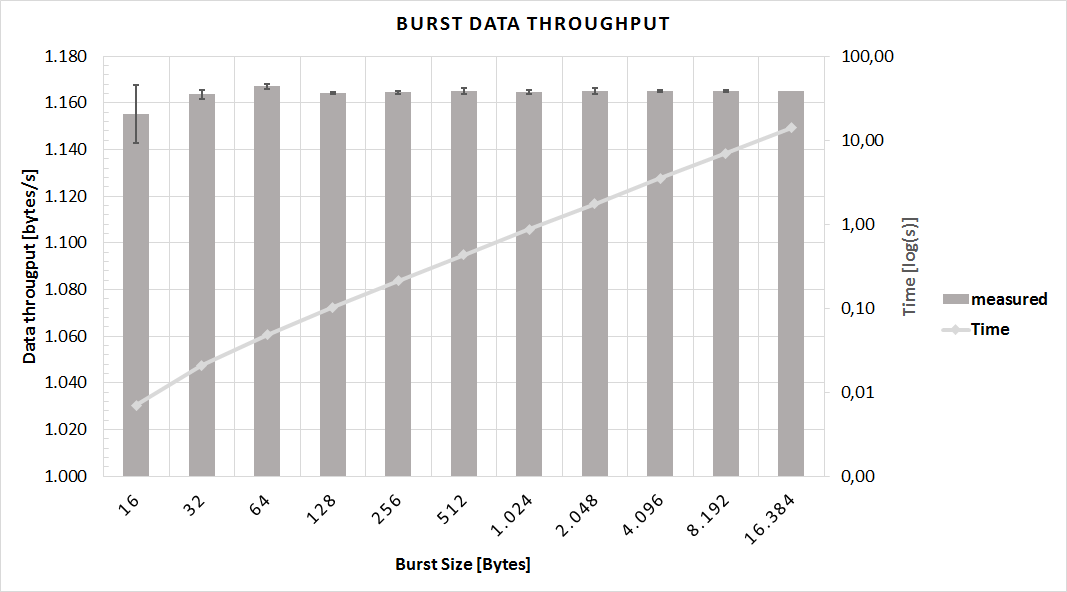
\includegraphics[scale=0.5]{content/images/exp5.png}
		\caption{Burst data rate}\label{fig:exp5}
	\end{figure}
	Figure \ref{fig:exp5} shows the achieved data rates for the different packet sizes and also the length of the transfer. As seen the values all hover around the same value of ~1165 Bps. This is approximately the same value as the one which can be achieved with the other two types of data.
	Again see section \ref{sec:dataThrougput} for a discussion about possible reasons for this upper limit. 
\end{description}
\newpage

\section{Experiment 6: Maximum communication Range}
\begin{description} 
	\item{\textbf{Description}} \hfill \\  In this experiment we try to determine the correlation between the maximum range and the power setting of the ANT radio. One of SHAMPU's advantages is the low power consumption, so it might be possible to further reduce the power consumption by decreasing the power level of the ANT radio, especially in smaller environments where there is no need for such a range. According to the datasheet the maximum range for communication is 30m, however the ANT documentation does not provide different ranges for different power settings. 
	
	\item{\textbf{Use-Case}} \hfill \\ Unscheduled data-transmission and scheduled data-transmission	
	\item{\textbf{Network topology and pseudo code}} \hfill \\ 
	\begin{figure}[H]
		\centering
		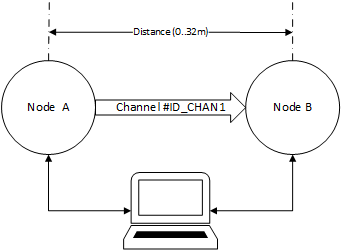
\includegraphics[scale=1]{content/images/exp6_topo.png}
		\caption{Topology experiment 6}
	\end{figure}
	
	\begin{code}[H]
		\begin{verbatim}
		for (pSetting in Available_PowerSettings)
		  ANT_SetTransmitPower(pSetting)
		  openChannel(ID_CHAN1, ANT_Bidirectional_Master)
		  ANT_SendBroadcastData(ID_CHAN1, [0x01, 0x02, 0x03, 0x04])
		  wait_for_user_input();
		  closeChannel(ID_CHAN1);
		\end{verbatim}
		\caption{Maximum communication range (Master)}\label{lst:mExp6}
	\end{code}
	
	\begin{code}[H]
		\begin{verbatim}
		distance = 0.0
		stopInc = false
		loop 
		  openChannel(ID_CHAN1, ANT_Bidirectional_Slave)
		  wait_until(received_Packet == ANT_BROADCAST_DATA || 
		             received_Packet == ANT_MESSAGE_EVENT_RX_SEARCH_TIMEOUT) 
		  if (stopInc) 
		    if (wasTimeout) 
		      distance -= .4
		    else 
		      print "Connection found : " + distance
		  else
		    if (wasTimeout)  
		      stopInc = true
		      distance -= .4
		      print "Connections lost : " + distance
		    else distance += .4
		  closeChannel(ID_CHAN1);
		\end{verbatim}
		\caption{Maximum communication range (Slave)}\label{lst:sExp6}
	\end{code}
	\item{\textbf{Testing methodology}} \hfill \\ At the beginning of the experiment Node A and B are placed right next to each other. Node A acts as a master and keeps broadcasting the same message. Node B is the slave and tries to connect to the channel. If the connection is successful, the distance between the two nodes is increased by 0.4 meters. This process is repeated until Node B can no longer connect to the channel and the connection times out. This happens after 30s of searching. At this point the distance is no longer increased, but rather decreased until Node B is able to successfully connect to the channel. Both of these values are recorded. The whole experiment is then repeated for each available power setting.	
	\newpage
	\item{\textbf{Result}} \hfill \\ 
	\begin{figure}[H]
		\centering
		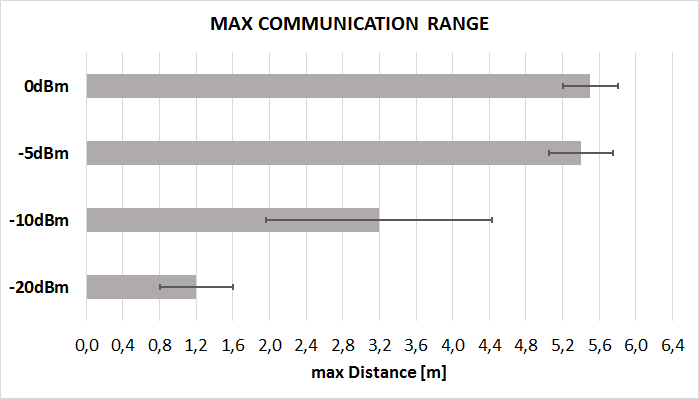
\includegraphics[scale=0.5]{content/images/exp6.png}
		\caption{Maximum comunication range}\label{fig:exp6}
	\end{figure}
	Figure \ref{fig:exp6} shows the transmission range for each power setting. As expected the maximum distance goes up with the higher power settings. But the result at the highest power setting is disappointing, since we did not get close to the claimed maximum range of 30m. The ANT documentation states that the maximum range of 30m can only be achieved in "optimal conditions" \cite{DynastreamInnovationsInc.2013}. It is possible for several different unfavorable factors to interfere with the ANT signal, such as multiple 802.11 networks in the vicinity, or even the plastic case of the base station. 
\end{description}


\section{Maximum Data Throughput}
\label{sec:dataThrougput}

In our experiments we were able to confirm two important limits for the maximum data throughput which can be achieved with our current set up. The ANT AP1MxIB supports a maximum message frequency of 200 Hz, which means that we would expect to see a maximum transmission rate of 1600 Bps.
However, this limit can only be achieved by splitting the available bandwidth between receiving and sending. If we try to utilized the full 200 Hz only for either receiving or sending, we are limited to 1100 Bps, around 500 Bps or 30\% lower than the theoretical maximum. The same 1100 Bps limit holds for burst transmissions, where we loose around 1100 Bps or 56\% of the maximum data throughput.\\

To balance environmental influences, the experiments were repeated in different locations and times of day and night. Since the throughput did not change noticeably, it can be assumed that there are no easily eliminated environmental factors which affect the maximum rate. We conclude that the root cause for the lower than expected throughput must be attributed to the hardware or software. \\

If we exclude environmental factors, we are left with three possible reasons:
\begin{itemize}
	\item{\textbf{RS-232 Connection}} \hfill \\ The base station is connected to a PC over a serial connection. For the speed we chose 19200 baud, since it is the highest value supported by the ANT chip and the serial-Interface. With 19200 baud the maximum data rate of the RS-232 Connection is 1920 Bps, since the interface adds a start and stop bit to each byte. This data rate is enough for the maximum message frequency. If the serial connection would be the bottle neck for burst transmission, we would expect to be able to atleast get the full 1920 Bps as data throughput. Since this is not the case we can conclude that the RS-232 connection has no negative effect on the data throughput.

	\item{\textbf{ANT API}} \hfill \\ The software we use is not officially supported by ANT. It is thus possible that there are some bugs which have an impact on the performance. Except for the missing burst mode (see \ref{sec:future}), there were no unusual measured values during the experiments. If there is a bug, it might be hard to find without rewriting all the experiments and running them with the official ANT library \cite{ANTWinLib}
	
	\item{\textbf{ANT AP1MxIB}} \hfill \\ Due to the black box nature of ANT, it is very hard to exactly determine what causes the problem. The inner workings of the chip are not documented in any way, and the error messages of the protocol are not very specific. We suspect that the ANT chip receiver and sender are somehow limiting the maximum data throughput. The chip itself is from 2007 and the manufacturer no longer recommends the use of the chip\cite{AP1page}. There are alternatives available, like the newer ANTAP281M5IB chip \cite{AP2Datasheet}.
\end{itemize}
\newpage	%Evaluation of SHAMPU
\chapter{Conclusion}


\section{Summary}
In conclusion of our experiments, it seems af if the ANT chip falls short of its full potential:
\begin{itemize}
	\item{\textbf{Scheduled data-transmission}} \hfill \\ The achieved data throughput of around 1160 Bps is valid for a single chip. That means the main bottleneck of the network is the base station, since it acts as a command and control server for each node in the network. The easiest way to fix the problem is to use more than one base station. This is possible, since we do not need a fully meshed network for the SHAMPU nodes to communicate with each other. They solely need to talk to the base station.
	
	\item{\textbf{Unscheduled data-transmission}} \hfill \\ The achievable burst data throughput is especially problematic. SHAMPU is equipped with 128 kBytes of RAM. With the current set up it takes about 2 minutes to dump the entire memory to a base station, where is can be further analysed. If the full potential of the burst mode could be made available, the duration can be shortened to 70s. The long burst duration poses a problem, as long bursts disrupt the communication on other channels. For this reason the transmission of these memory-dumps has to be very carefully scheduled to avoid network congestion.
	
	\item{\textbf{Communication Range}} \hfill \\ The maximum achieved range of 6m is probably the most disturbing result of this thesis. The short range signifies, that the physical location of the base station is critical for a successful deployment of SHAMPU. It also means that a larger network requires more than one such base station to be able to reach all nodes.
\end{itemize}


With all these limitations of the data throughput, the network setup has to be chosen very carefully. One option is to use additional SHAMPU nodes as relays, which serve a dual purpose. They allow to extend the range of the network, while increasing the data throughput of the whole network.\\ Another possibility to counteract the limitation is to leverage the numerous advantages of the SHAMPU framework, such as its low weight, form factor and power draw. A mobile base station, e.g. TrainSense \cite{smeets2013trainsense}, which can easily be moved around in the location where the SHAMPU nodes are deployed, makes it possible to address all above mentioned problems. The range no longer represents a problem, since the base station is simply moved towards the node until a connection can be achieved. At the same time, the limited range provides a solution for the limited data throughput. Since the amount of nodes, which are able to connect to the base station can be controlled its possible to only ever have a small number of nodes transmitting data to the base station.

In the end, while ANT is not the most powerful wireless solution available, its design choices (low power consumption and ease-of-use) coincide almost completely with the design goals of SHAMPU.
\newpage
\section{Future Work}
\label{sec:future}
Due to lack of time and the limited hardware availability we were not able to fully explore and evaluate the ossibilities of ANT in the SHAMPU network. Especially the following four areas should be revisited:

\begin{itemize}
	\item{\textbf{Power consumptions}} \hfill \\ Each experiment tries to find the maximum of either data throughput or the communication range. We did not measure how the power consumption changes if, for example, the message period is reduced. Since SHAMPU tries to be very low-powered, this is an important measurement for the decision whether or not SHAMPU can be used for a specific application. The data sheet of the ANT AP1MxIB module provides interesting data \cite{Networks}: The maximum current draw seems to be around 5 mA for a continuous burst transmission and around 40 $\mu$A for a normal broadcast operation.
	
	\item{\textbf{Burst mode}} \hfill \\ We use a custom library, which provides an API to interface with the ANT-Chip. For this thesis an attempt was made to add the missing burst transfer mode. However, due to time constraints we were unable to get the mode working correctly. Burst packets need to have a precise timing, but the black box nature of the ANT protocol makes it a challenge to debug the code.
	
	\item{\textbf{Shared channels}} \hfill \\ Due to missing hardware, we were only able to test the communication between two nodes. Shared channels could not be tested, yet we expect the available data throughput to be in line with the results from our experiments. ANT uses up to 2 bytes of the 8 byte payload to specify the address of the receiver. Therefore we expect to lose approximately 12.5\% to 25\% of throughput if shared channels are used. It would be important to confirm this to fully assess the usefulness of the ANT chip.
	
	\item{\textbf{New ANT-chip}} \hfill \\ As mentioned before the chip currently in use is old and no longer recommended for use. The successor of the current chip, the ANTAP281M4IB has roughly the same specifications as the current chip. Therefore the experiments should be rerun with the newer model in order to determine whether the ANT-chip is the limiting factor for data throughput.
\end{itemize}
 %Discussion

% Appendix chapters to be put here. They will be enumerated with capital letters 
% if you  did not change the \documentclass options.
\begin{appendix}
\chapter{Sourcecode}

\lstinputlisting[language=C]{content/source/main.c}
\newpage
\lstinputlisting[language=C]{content/source/experiment.h}
\newpage
\lstinputlisting[language=C]{content/source/experiment.c} % Sourcecode

%\include{appendix_chapterA}
\end{appendix}
%Ende Anhang

%Bibliography
% We strongly recommend to use bibtex to manage your bibliography. It helps you
% structure your references and helps avoiding missing important data for a correct
% quotation. If you have no other idea jabref (http://jabref.sourceforge.net/)
% might be a good idea (Jave runtime environment needed).
% This style is good to use in german master thesis'. You need to have activated
% \usepackage{bigerm} above.
% For english documents just use apalike.
\bibliographystyle{unsrt}

% to finally announce where your bibliography is stored use
\bibliography{content/references/references}
%pagenumbering{null}

\ 

%clearpage
\cleardoublepage

\ 


\pagestyle{empty}
\vfill
\textbf{Erkl�rung}\\

\[German\] Hiermit versichere ich, dass ich die vorliegende Bachelorarbeit selbst�ndig verfasst, keine anderen als die angegebenen Quellen und Hilfsmittel benutzt, sowie Zitate kenntlich gemacht habe.\\

\[English\] I hereby declare that I have written this Bachelor thesis independently, using no other than the specified sources and resources, and that all quotations have been indicated.\\
\\\\
Essen, \today\\
$\overline{\parbox{3.5cm}{(Place, Date)}} ~~~~~~~~~~~~~~~~~~~~~~~~~~~ \overline{\parbox{4cm}{\studentFirsName { } \studentSecondName}}$
 %It may be necessary that you replace "Bachelorarbeit" with "Masterarbeit" here...

\end{document}
